
\documentclass[]{article}
\usepackage{graphicx}
\usepackage{color}
%opening
\title{MetaTracts - A Method for Robust Extraction and Visualization of Carbon Fiber Bundles in Fiber Reinforced Composites: Rebuttal}
\author{}

\begin{document}

\maketitle


\section{Reviewer 1}
\color{red}
Q1. A new variable, reliable Hessian, is defined and it is stated that $R_{H}$ is similar to the "vesselness".  Later on, the authors claim "the utility of the vesselness is a little different from our framework". Matching term by term between the definitions of "vesselness" and $R_{H}$, they are the same. The authors are encouraged to state clearly the originality and contribution of $R_{H}$.
\color{black}

A1. Reliable Hessians is computed exactly equivalently to Vesselness for a single scale (Firangi et al.~\cite{Frangi1998}). We have  updated the corresponding sentence in the paper to reflect the same. We explain further about the utility being different.


A common approach and one utilized by the Frangi et al.~\cite{Frangi1998}, is to consider the Taylor series expansion in the neighborhood of point $x$ in an image as.
\begin{equation}
f(x) = \sum_{i=0}^{\infty}\frac{f^{(i)}(0)}{i!}x^{i}
\end{equation}
The expansion often is approximated till the second order (Hessian). In particular the hessian maps a  neighborhood  centered about $x$ onto an ellipsoid  whose axes are along the directions given by the eigenvectors of the Hessian and the corresponding axis' semi-lengths are the magnitudes of the respective eigenvalues. Vesselness measure as described in the paper takes into account geometric ratios based on this and acts as a filtering process which searches for geometric structure that can be tubular. Figure~\ref{fig:Vesselness} shows results from Frangi et al.~\cite{Frangi1998} paper. Others including Sato et al.~\cite{Sato1997} have used the eigen decomposition to filter images.

As mentioned in the paper, we do not have clear tubular structures embedded in a dark contrast matrix such as in blood vessels ( Figure~\ref{fig:data-char-rebuttal} shows the data characteristics for our case.). Instead  the utility of $R_{H}$ is  to associate each grid location with a reliability measure for the local orientation as given by the  principal eigenvector. We use this orientation vector to create MetaTracts.

\begin{figure}
\centering
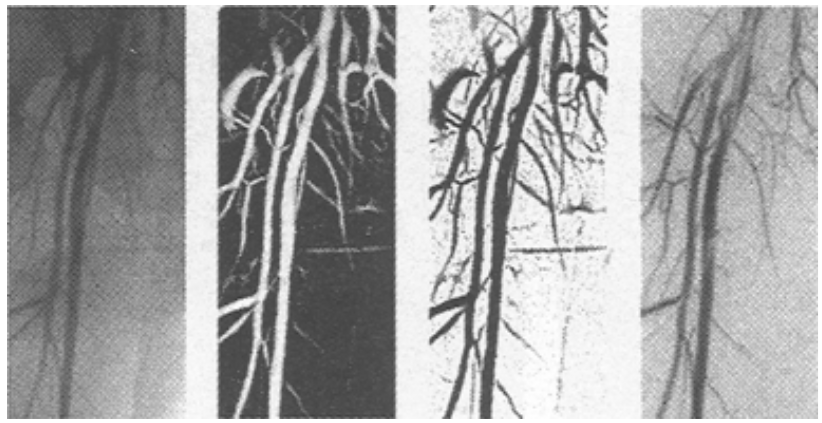
\includegraphics[width=0.7\linewidth]{images_pvis/Vesselness}
\caption{Left: Xray image of vasculature, middle-left: calculated vesselness of the left image, middle-right: calculated vesselness after inversion of the grey-scale map. Right image after subtracting reference from left image.}
\label{fig:Vesselness}
\end{figure}

\begin{figure}[tb]
	\centering
	%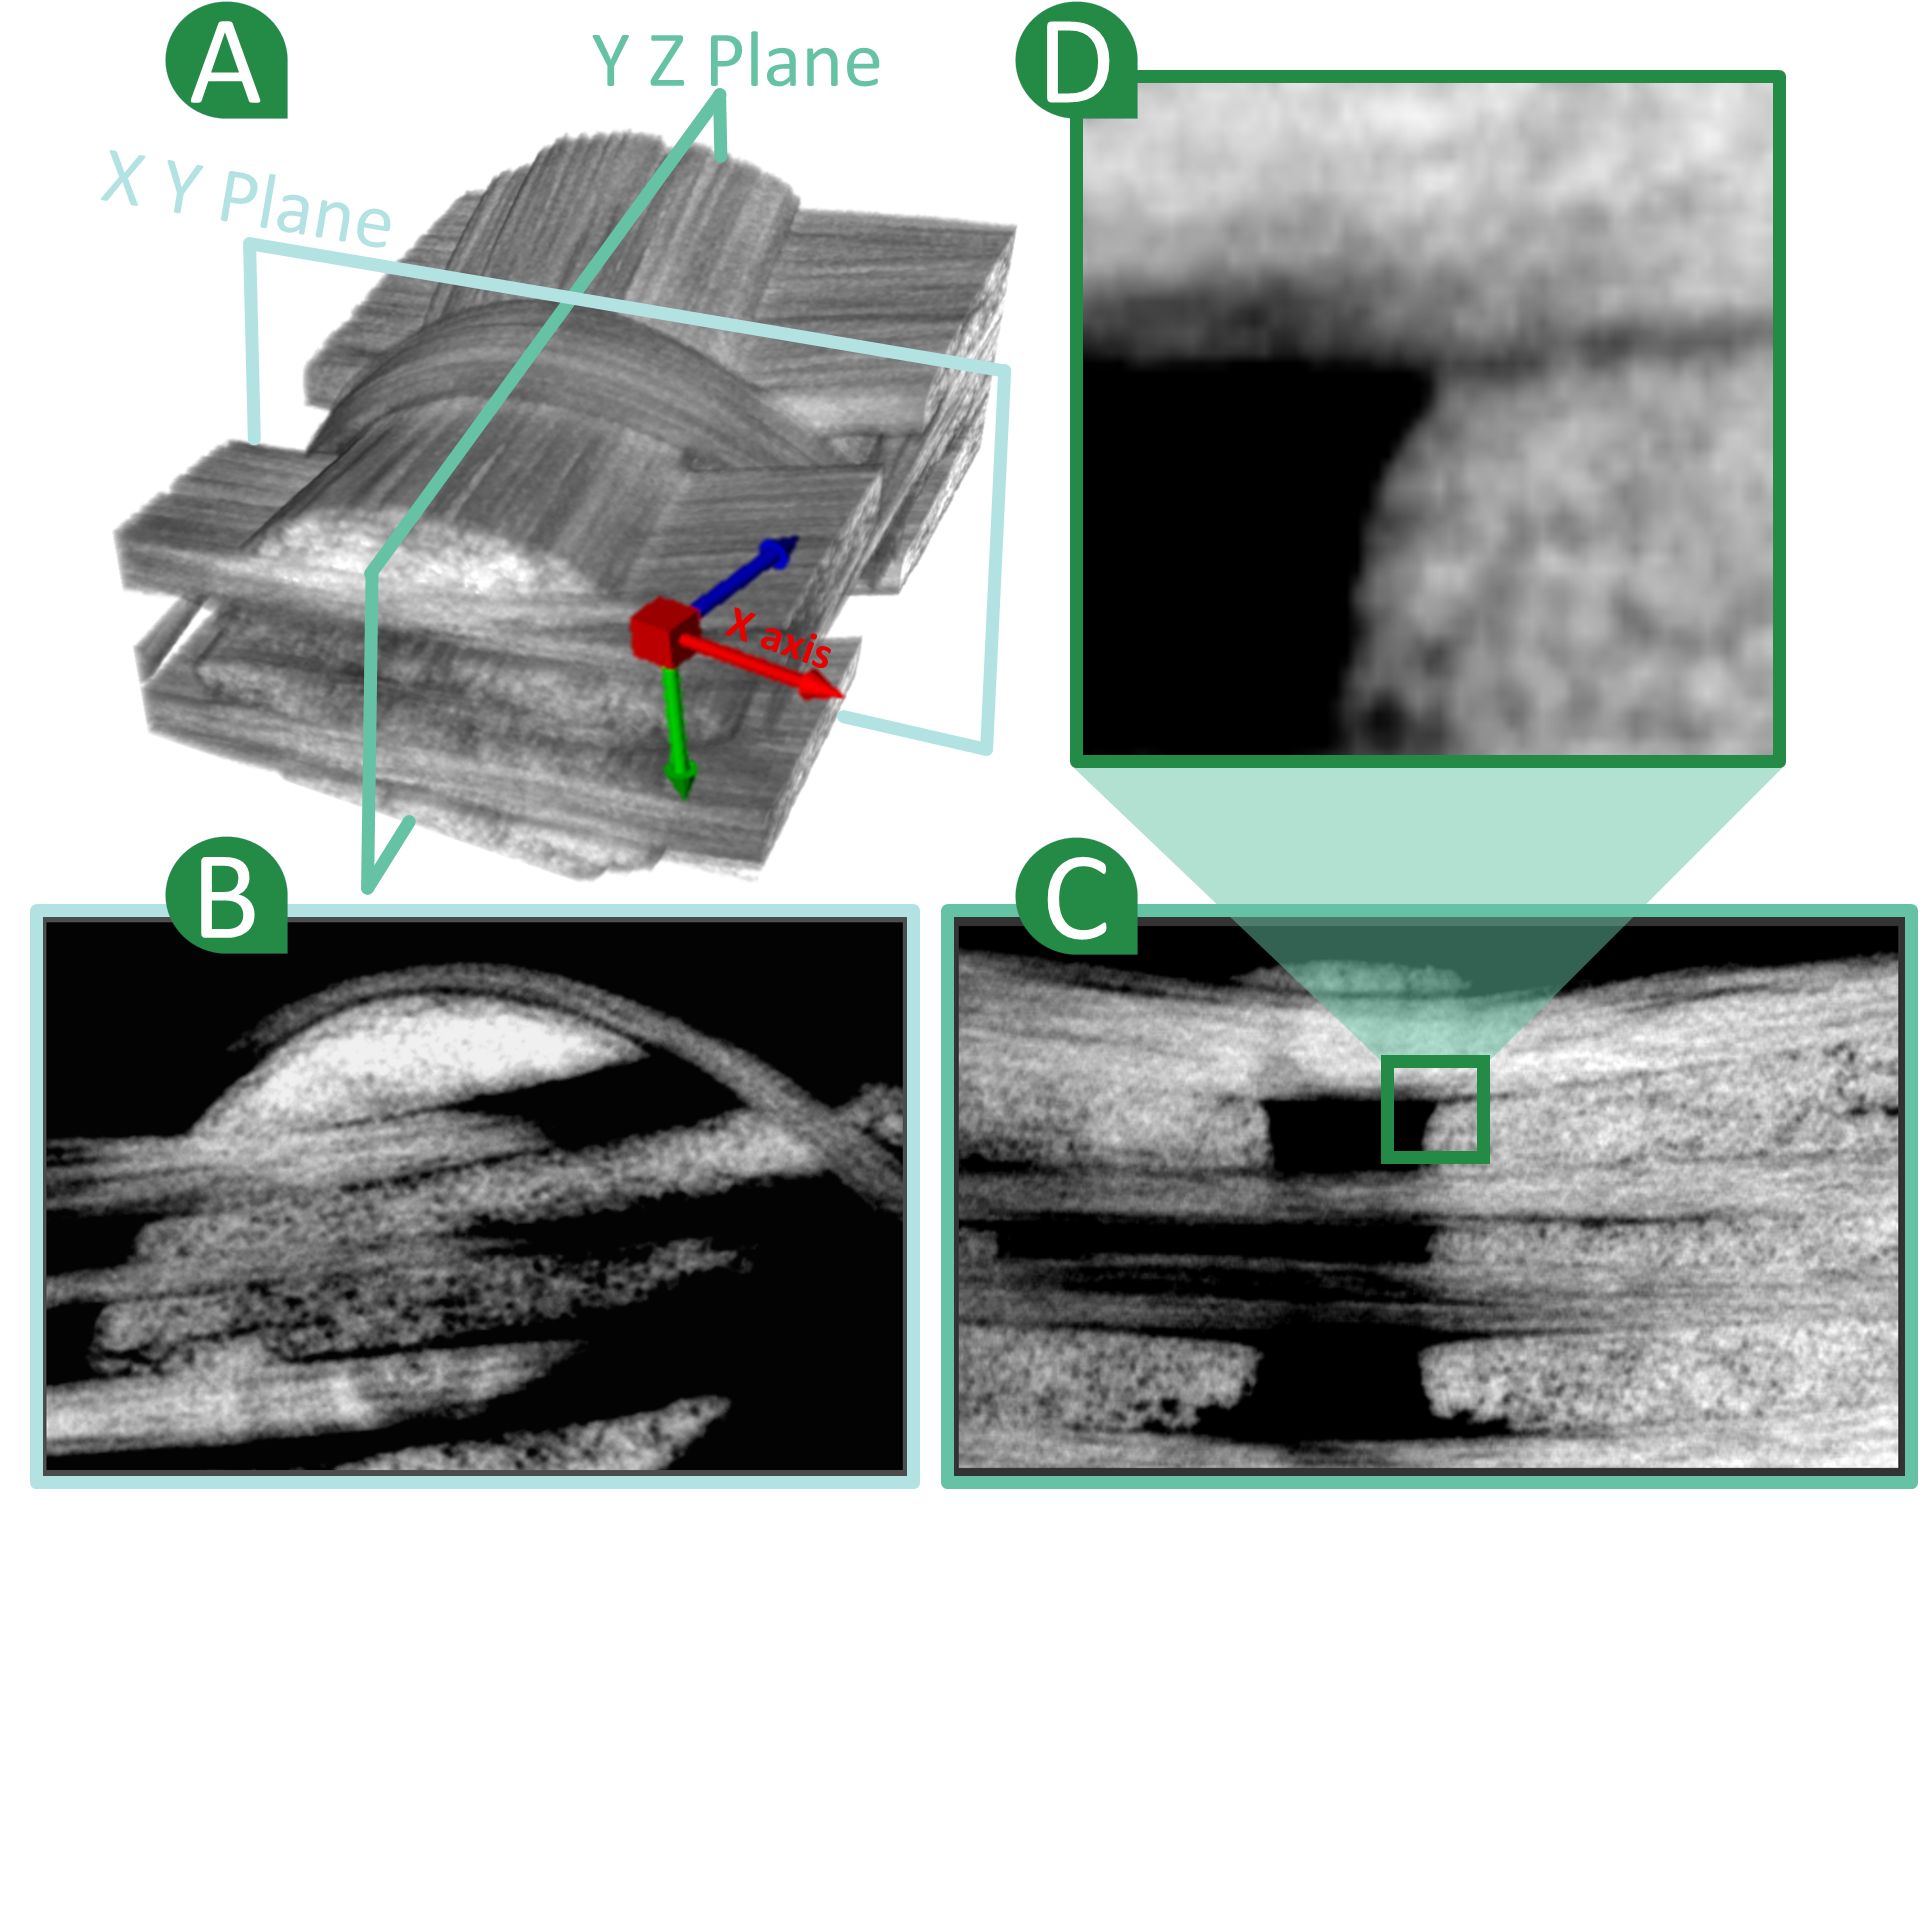
\includegraphics[width=0.5\textwidth, trim = 0mm 110mm 0mm 0mm, clip,]{images_pvis/figure1}
	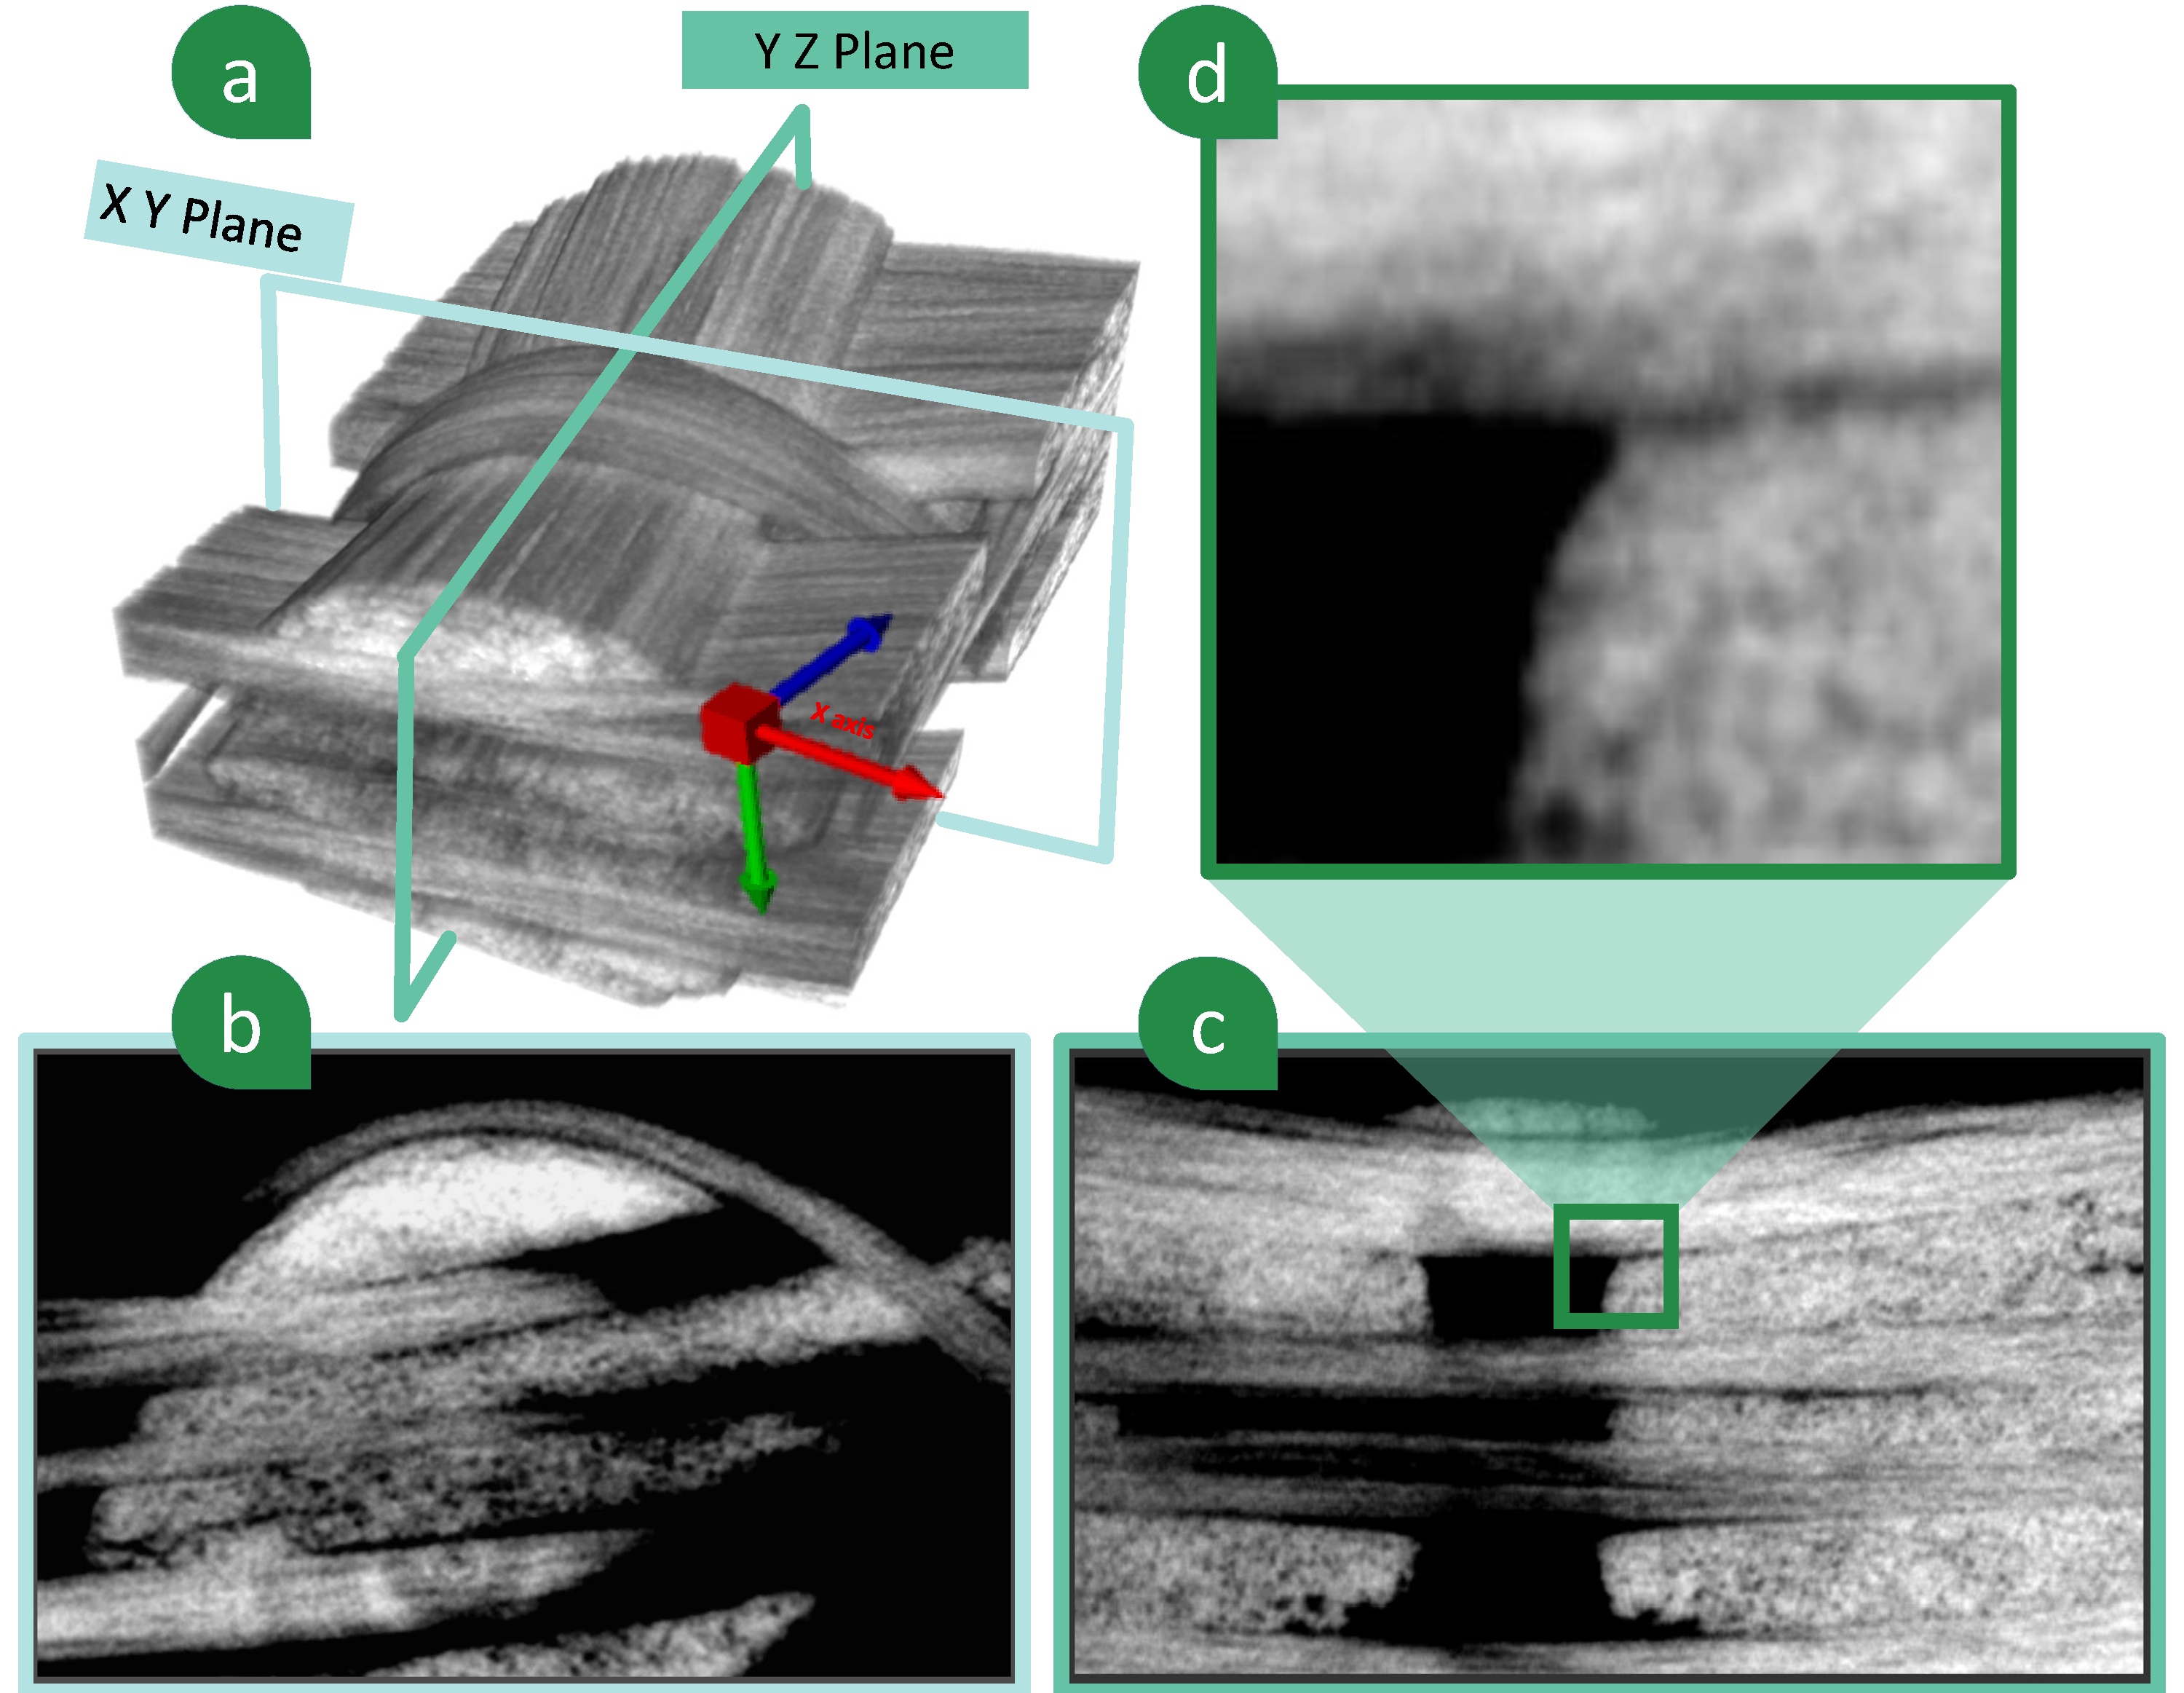
\includegraphics[width=\linewidth]{images_pvis/data-char.pdf}
	\caption{Data characteristics: (a) Rendering of the data. (b) 2D slices along the X-axis and (c) 2D slice along the Z-axis. (d) Magnified region marked in green square (c). Multiple fiber bundles cross and are indistinguishable by visual inspection alone. }
	\label{fig:data-char-rebuttal}
\end{figure}

\color{red}
Q2. In the examples presented, it seems only one type of composite was studied. For instance, there is no example showing a composite with fiber bundles that cross each other at an angle $<$ 90 degrees. When two bundles are almost parallel, will the current algorithm be sufficient to separate them apart? The authors are encouraged to provide more than one fiber configurations.
\color{black}

Answer. Due to the manufacturing process, a vast majority of composites have bundles crossing at ~90 degree angles. With the separation factors being width, spacings and compactness of fiber bundles. These variations are well represented in our data sets. We maintain that the technique is useful and applicable to a large percentage of composite polymers. Nevertheless, we have added a third dataset in the supplementary materials which will be included in a comprehensive technical report which we cannot add currently due to space restrictions.

Figure~\ref{fig:angle_bundles}f, bundles 7,10 and 6 shows a common example of variations in the datasets which we extract accurately. 
\begin{figure}
\centering
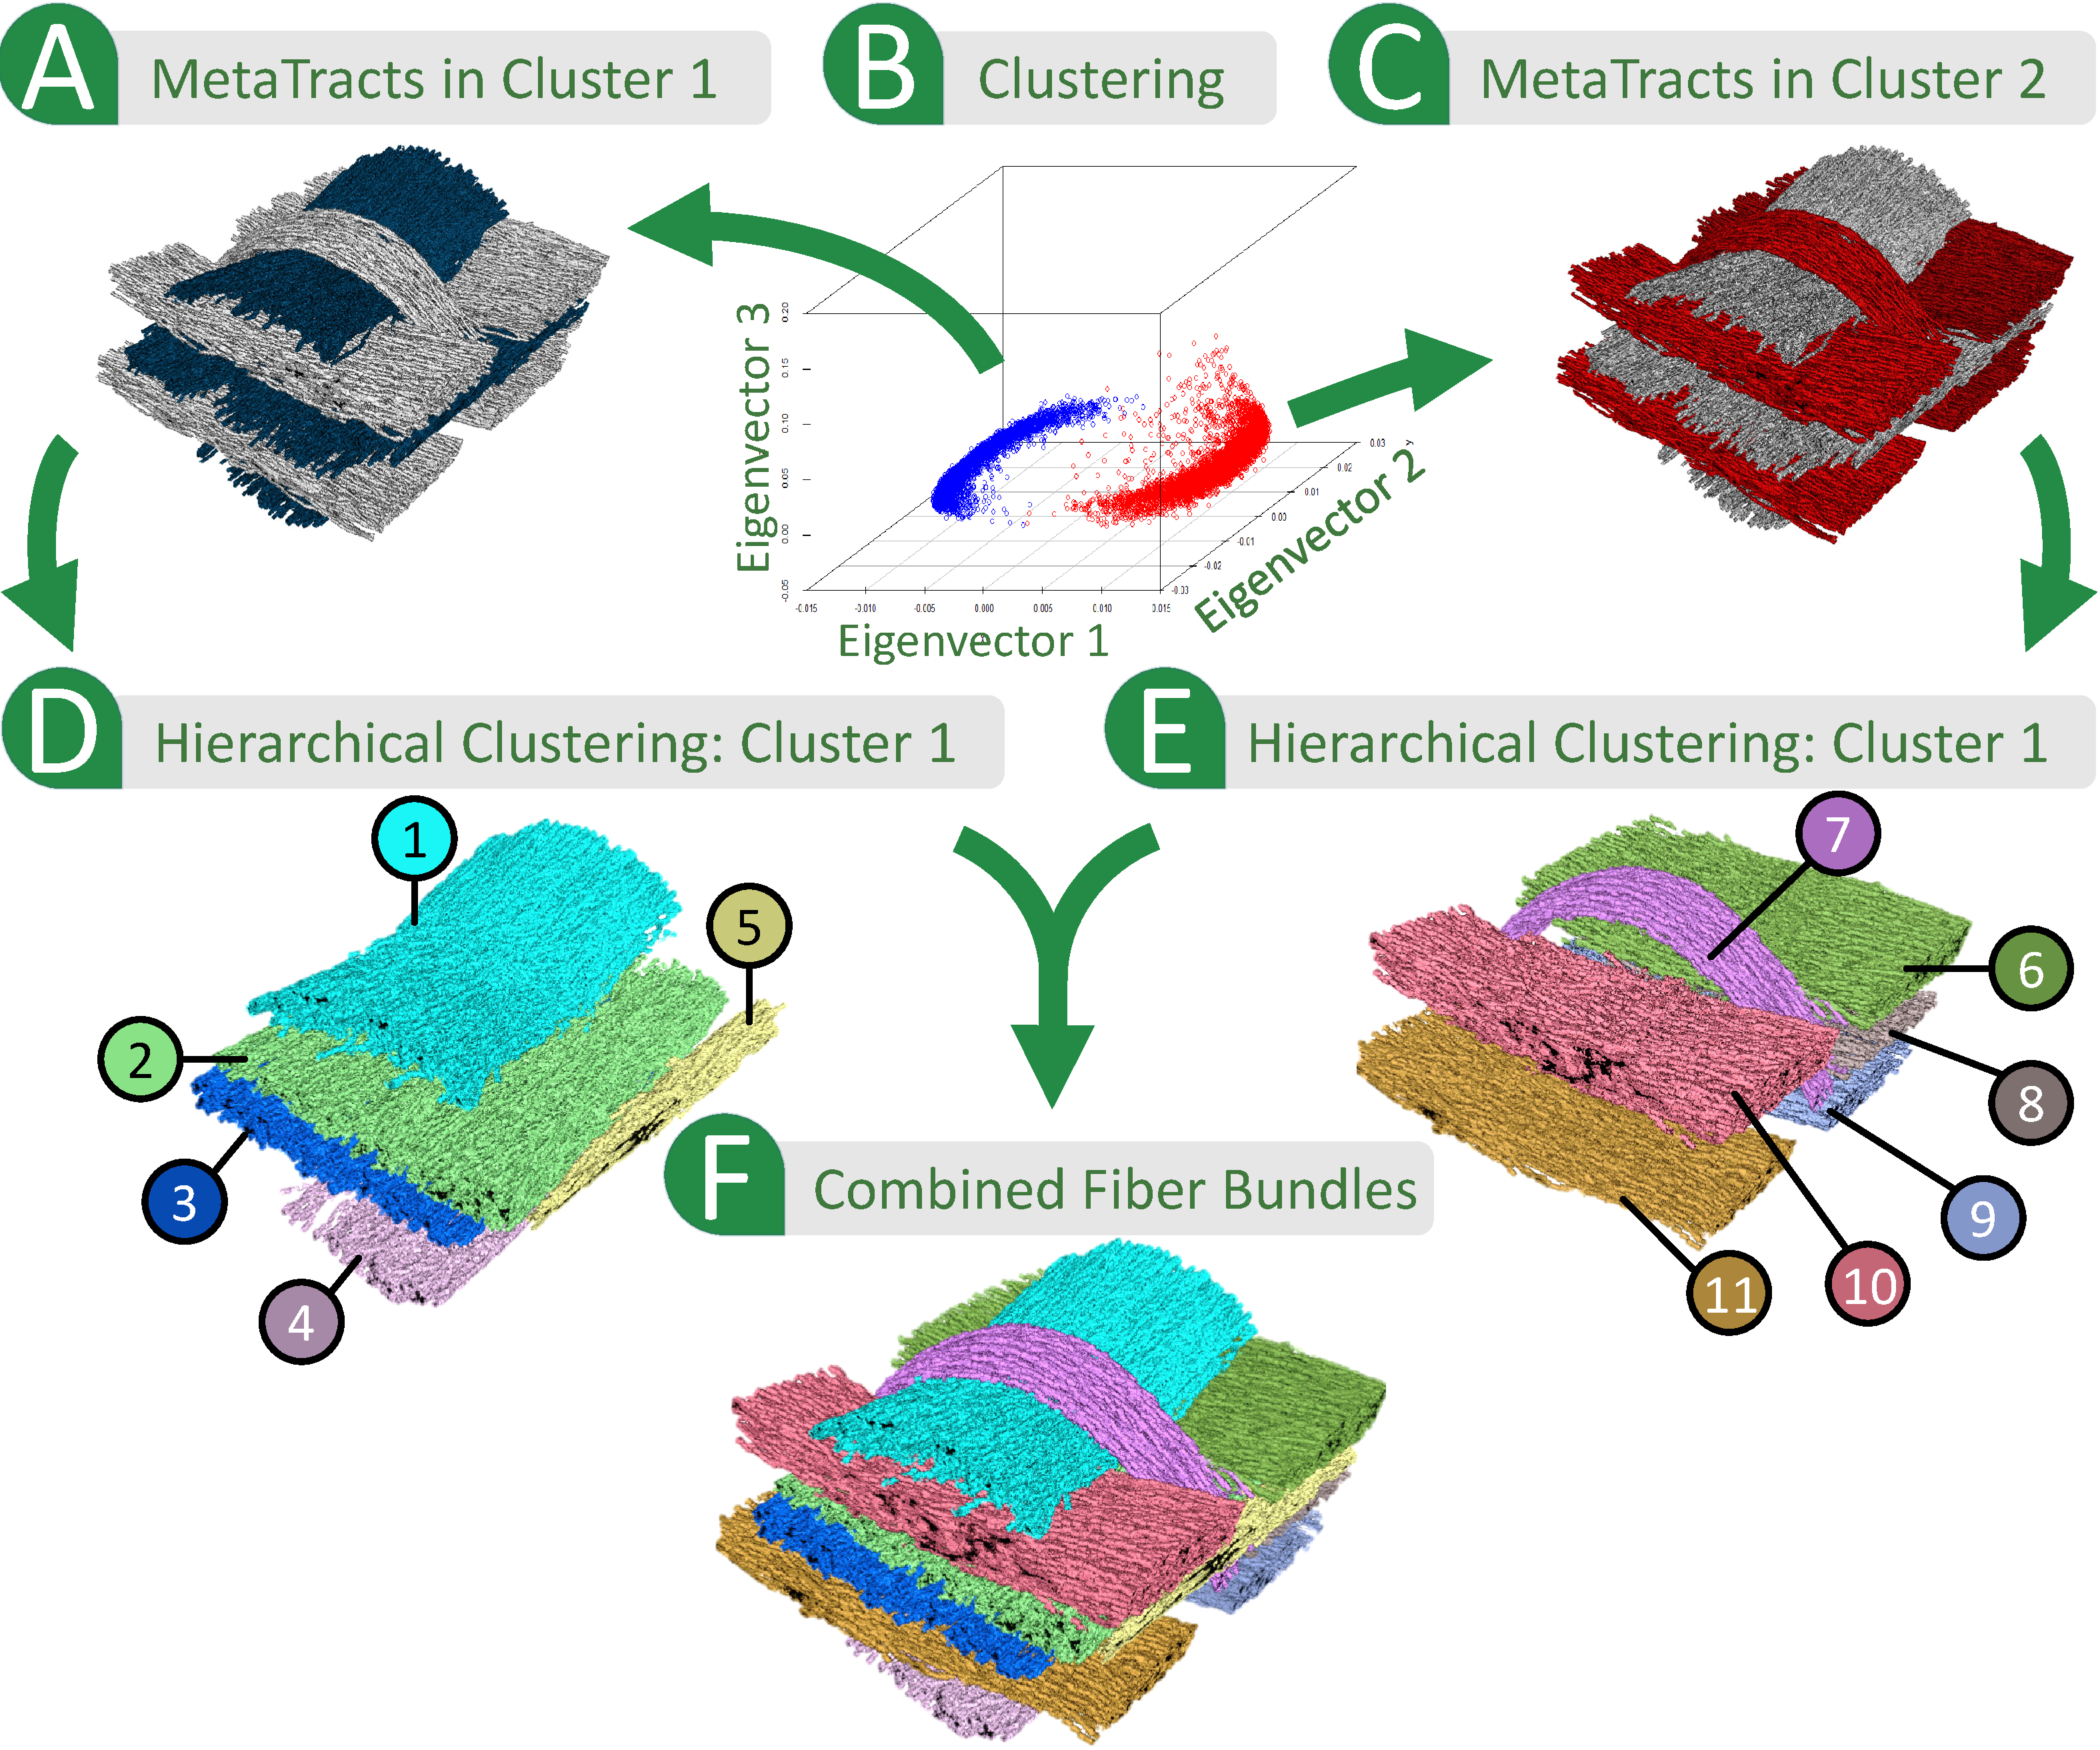
\includegraphics[width=0.7\linewidth]{images_pvis/clustering.pdf}
\caption{Fiber bundles extraction}
\label{fig:angle_bundles}
\end{figure}
  

\color{red}
Q3. All clustering was done in R. The letter R is not explained.
\color{black}

A3. R is a free software environment for statistical computing and graphics.

\section{Reviewer 2}
\color{red}
I feel the background section could be improved. Why the orientation and weaving patterns of fibers indicate the strength of the material, and thus why the trouble to scan the materials, extract the fibers and visualize them. The paper gives some relatively high-level description of this but more background would be appreciated.


\color{black}
Answer.

\color{red}
  It seems to me that the extracted fibers may not be real fibers. Is this
  true? If so, how well can one trust the weaving patterns extracted based
  on the imaginary fibers? 
  \color{black}
  Answer. 
Yes, the extracted fibers cannot be mapped to real fibers. One of the goals  we  focused on was to move away from extraction of individual fibers, instead work on direct reconstruction of bundles. The design decisions adheres to extracting reliable bundles directly from the images. 
 Developing methods which can precisely compute the deviations from original bundles remains a future direction of the project. 

\color{red}
The authors claim that their method can deal with low resolution data.
But this might be in the eyes of the beholders, since in my opinion the example data in the paper all have fairly high resolutions. Perhaps a comparison with a really high resolution data using this method and other existing methods could diffuse the doubt.
\color{black}

Answer. Figure~\ref{fig:glass_fibers} shows an example where each fiber is clearly demarcated compared to the type of data we address in the paper (Figure~\ref{fig:data-char-rebuttal}).
\begin{figure}
\centering
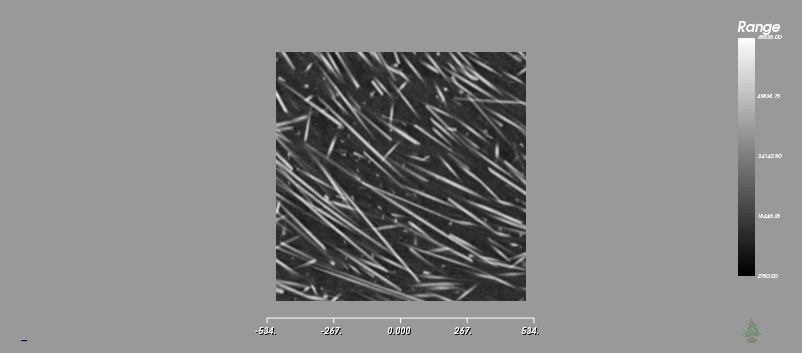
\includegraphics[width=0.7\linewidth]{images_pvis/glass_fibers}
\caption{High Resolution fiber}
\label{fig:glass_fibers}
\end{figure}


\section{Reviewer 4}
\color{red}
In Section 5.1, k-means is applied to the m-dimensional space using
Euclidean distance, i.e., each dimension is considered equally important.
Is that really the case when they represent eigenvectors?

\color{black}
Answer. Belkin  and Niyogi's~\cite{Belkin01} laplacian eigenmaps embeds the high dimensional data ( represented as a graph ) into a low dimensional space where the Euclidean distance approximates the distances in higher dimension space. For such reason, Eigen embedding for dimensionality reduction has become quiet popular and has found favor in tackling a variety of problems. Empirically the K-means for orientation clustering provided us excellent results. The major orientations are limited by the inherent characteristics of our data set and this also plays a role in Laplacian embedding followed by k-means giving us such good results. A formal proof is not provided. 

\color{red}
In Section 5.2, the authors mention that they remove short Meta Tracks.
How much data is thrown away here? Can examples be provided to get a
better understanding?
\color{black}


\color{red}

What are the limitations of the approach? Are there data sets where the
method fails?
\color{black}
Answer. We have added a ``Limitations and future work" Section to the end of the paper. We copy it here for completeness.


 A key assumption of the method is ``connectivity'' (Sec. Data Characteristic).
 If the ``connectivity'' is not satisfied due to noise in the image, the then MetaTracts will be inaccurate. 
 The clustering process also assumes that the fiber bundles have a minimum width. 
\bibliographystyle{abbrv}
%%use following if all content of bibtex file should be shown
%\nocite{*}
\bibliography{xBundle}
\end{document}
